\chapter{Tercera ley de la termodinámica}

\section{Postulado de Nernst--Planck}

\begin{postulado}[IV: Planck--Nernst]
  La entropía de cualquier sistema dado se anula en el estado para el cual se cumple que
  \begin{equation*}
    \pdvc{U}{S}{V,N_1,\dots,N_r}=0\qquad(\text{implica }T=0),
  \end{equation*}
  (después veremos por qué). Es decir,
  \begin{equation*}
    \lim_{T\to0}S=0,\qquad S=0\;\Longrightarrow\;T=0.
  \end{equation*}
\end{postulado}

Esto es conocido como \textbf{postulado de Planck--Nernst} (Walther Nernst y Max Planck) o
\textbf{tercera ley de la termodinámica}. Este postulado implica que existe un estado donde $T=0$
(cero absoluto). Sin embargo, puede ser violado por sistemas cuánticos o no extensivos
(gravitacionales).

Este postulado fue la última ley de la termodinámica en ser desarrollada y es incompatible con la
mecánica estadística clásica, por lo que requiere de la introducción de la mecánica estadística
cuántica.

Estos cuatro postulados forman las bases lógicas de la termodinámica clásica (no confundir con las
leyes de la termodinámica).

\subsection*{Ejercicios}

\begin{ejercicio}
  Las siguientes relaciones son aparentemente relaciones termodinámicas fundamentales; sin embargo,
  puede ser que algunas de ellas sean inconsistentes con los postulados I--IV y, por lo tanto, no
  sean físicamente aceptables. En cada caso dibuje cualitativamente la relación entre $S$ y $U$
  (con $N$ y $V$ constantes). Las cantidades $v_0$, $\theta$ y $R$ son constantes positivas. En
  aquellos casos donde aparecen exponentes fraccionarios, tome únicamente las raíces positivas.
  Además, si la relación es físicamente aceptable, encuentre $U(S,V,N)$.
  \begin{enumerate}[label=\alph*),itemsep=2pt]
    \item $\displaystyle S=\left(\frac{R}{v_0\theta}\right)^{\!1/3}(NVU)^{1/3}$.
  \end{enumerate}
\end{ejercicio}

\begin{solucion}
  \begin{enumerate}[label=\alph*),itemsep=2pt]
    \item El postulado I se cumple (estados de equilibrio de $N,V,U$) y el postulado II se cumple
      ($S=S(U,V,N)$). Para el postulado III,
      \begin{align*}
        S(\lambda U,\lambda V,\lambda N)&=\left(\frac{R}{v_0\theta}\right)^{\!1/3}(\lambda N\cdot\lambda V\cdot\lambda U)^{1/3}
          =\left(\frac{R}{v_0\theta}\right)^{\!1/3}(\lambda^{3}NVU)^{1/3}\\
        &=\lambda\left(\frac{R}{v_0\theta}\right)^{\!1/3}(NVU)^{1/3}=\lambda\,S(U,V,N),
      \end{align*}
      por lo tanto se cumple que es homogénea de orden $1$ (aditiva $\to$ extensiva). Con $U>0$ (en
      todos los casos), si se grafica $S$ vs.\ $U$ para $N$ y $V$ constantes se obtiene $S\propto U^{1/3}$.
      \begin{figure}[H]
        \centering
        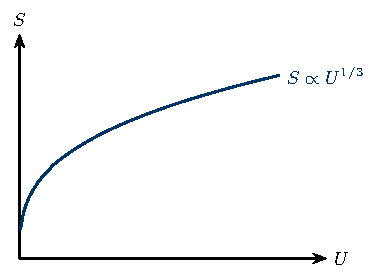
\includegraphics{figuras/S-U-tercio.pdf}
      \end{figure}
      Por lo tanto $S$ es creciente y monótona, continua y diferenciable, y
      \begin{equation*}
        S=\left(\frac{R}{v_0\theta}\right)^{\!1/3}(NVU)^{1/3}
      \end{equation*}
      es una relación fundamental. Invirtiendo $S$: elevando al cubo,
      \begin{equation*}
        S^{3}=\frac{R}{v_0\theta}\,(NVU)
        \quad\Longrightarrow\quad
        \left(\frac{v_0\theta}{R}\right)S^{3}=NVU
        \quad\Longrightarrow\quad
        \boxed{U=\left(\frac{v_0\theta}{R}\right)\frac{S^{3}}{NV}}
      \end{equation*}
    \item $\displaystyle S=\left(\frac{R}{\theta^{2}}\right)^{\!1/3}\left(\frac{NU}{V}\right)^{2/3}$.
      Revisando cada postulado: el postulado I se cumple ($U,V,N$ son variables de bulto) y el
      postulado II se cumple ($S=S(U,V,N)$). Para el postulado III,
      \begin{align*}
        S(\lambda U,\lambda V,\lambda N)&=\left(\frac{R}{\theta^{2}}\right)^{\!1/3}\left(\frac{\lambda N\cdot\lambda U}{\lambda V}\right)^{2/3}
          =\left(\frac{R}{\theta^{2}}\right)^{\!1/3}\left(\lambda\,\frac{NU}{V}\right)^{2/3}\\
        &=\lambda^{2/3}\left(\frac{R}{\theta^{2}}\right)^{\!1/3}\left(\frac{NU}{V}\right)^{2/3}=\lambda^{2/3}\,S(U,V,N),
      \end{align*}
      por lo que el postulado III \textbf{no} se cumple y $S$ no es aditiva ni extensiva. La gráfica
      de $S$ vs.\ $U$ es $S\propto U^{2/3}$.
      \begin{figure}[H]
        \centering
        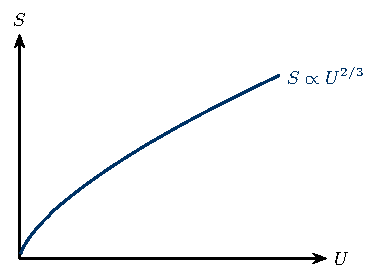
\includegraphics{figuras/S-U-dostercios.pdf}
      \end{figure}
      \textbf{No es una relación fundamental.}
    \item $\displaystyle S=\left(\frac{R}{\theta}\right)^{\!1/2}\left(NU+\frac{R\theta V^{2}}{v_0^{2}}\right)^{1/2}$.
      Los postulados I y II se cumplen ($U,V,N$; $S=S(U,V,N)$). Para el postulado III,
      \begin{align*}
        S(\lambda U,\lambda V,\lambda N)&=\left(\frac{R}{\theta}\right)^{\!1/2}\left[\lambda N\cdot\lambda U+\frac{R\theta}{v_0^{2}}(\lambda V)^{2}\right]^{1/2}
          =\left(\frac{R}{\theta}\right)^{\!1/2}\left[\lambda^{2}NU+\lambda^{2}\frac{R\theta V^{2}}{v_0^{2}}\right]^{1/2}\\
        &=\lambda\left(\frac{R}{\theta}\right)^{\!1/2}\left(NU+\frac{R\theta V^{2}}{v_0^{2}}\right)^{1/2}=\lambda\,S(U,V,N),
      \end{align*}
      por lo tanto $S$ es aditiva y extensiva. Con $U>0$, $S\propto U^{1/2}$, que es monótona y
      diferenciable.
      \begin{figure}[H]
        \centering
        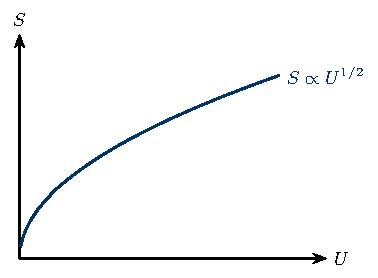
\includegraphics{figuras/S-U-mitad.pdf}
      \end{figure}
      Es una relación fundamental. Invirtiendo la relación, elevando al cuadrado,
      \begin{equation*}
        S^{2}=\frac{R}{\theta}\left(NU+\frac{R\theta V^{2}}{v_0^{2}}\right)
        \;\Longrightarrow\;
        \frac{\theta}{R}\,S^{2}=NU+\frac{R\theta}{v_0^{2}}V^{2},
      \end{equation*}
      \begin{equation*}
        NU=\frac{\theta}{R}\,S^{2}-\frac{R\theta}{v_0^{2}}\,V^{2}
        \;\Longrightarrow\;
        \boxed{U=\frac{\theta}{R}\,\frac{S^{2}}{N}-\frac{R\theta}{v_0^{2}}\,\frac{V^{2}}{N}}
      \end{equation*}
  \end{enumerate}
\end{solucion}

